\documentclass{scrreprt}

\usepackage{aligned-overset}
\usepackage{amsmath}
\usepackage{amssymb}
\usepackage{bm}
\usepackage[shortlabels]{enumitem}
\usepackage{hyperref}
\usepackage[utf8]{inputenc}
\usepackage{multicol}
\usepackage{mathtools}
\usepackage{physics}
\usepackage{tabularx}
\usepackage{titling}
\usepackage{fancyhdr}
\usepackage{xfrac}
\usepackage{pgfplots}

\pgfplotsset{compat = newest}
\usetikzlibrary{intersections}
\usetikzlibrary{patterns}
\usepgfplotslibrary{fillbetween}

\author{Karsten Lehmann}
\date{WiSe 2021/2022}
\title{Übungsblatt 01\\Lineare Algebra - Grundlegende Konzepte}

\setlength{\headheight}{26pt}
\pagestyle{fancy}
\fancyhf{}
\lhead{\thetitle}
\rhead{\theauthor}
\lfoot{\thedate}
\rfoot{Seite \thepage}

\begin{document}
\paragraph{Aufgabe 1:} Seien
$A \coloneqq \qty{x \in \mathbb{N} {\Big |} 10 < 2x^2 + 1 < 100}$,
$B \coloneqq \qty{x \in \mathbb{N} {\Big |} \abs{x - 7} \leq 3}$,
$C \coloneqq \qty{ 2z {\Big |} z \in \mathbb{Z}, z^2 \geq 4}$ und
$D = \qty{3, 4}$.

\begin{enumerate}[(a)]
\item Berechnen Sie die Mengen
  \begin{multicols}{3}
    \begin{enumerate}[(i)]
    \item $A \cup B$
    \item $B \cap C$
    \item $\mathcal{P}(B \cap C)$
    \item $A \times D$
    \item $(A \setminus B) \setminus C$
    \item $A \setminus (B \setminus C)$
    \end{enumerate}
  \end{multicols}

\item Für jede natürliche Zahl $n$ sei
  $M_n \coloneqq \qty{ m {\Big |} m \in \mathbb{N}, m \leq n }$.
  Bestimmen Sie
  \[
    \bigcup_{n \in \mathbb{N}}M_n \text{ und } \bigcap_{n \in \mathbb{N}} M_n
  \]
\end{enumerate}

\subparagraph{Lsg.}
\begin{enumerate}[(a)]
\item \begin{flalign*}
    A &= \qty{x \in \mathbb{N} {\Big |} 10 < 2x^2 + 1 < 100} &= &\qty{3, 4, 5, 6, 7} & \\
    B &= \qty{x \in \mathbb{N} {\Big |} \abs{x - 7} \leq 3} &= &\qty{4, 5, 6, 7, 8, 9, 10} \\
    C &= \qty{ 2z {\Big |} z \in \mathbb{Z}, z^2 \geq 4} &= & \qty{\ldots, -10, -8, -6, -4, 4, 6, 8, 10, \ldots} \\
    D & &=& \qty{3, 4}
  \end{flalign*}
  \begin{enumerate}[(i)]
  \item $A \cup B = \qty{3, 4, 5, 6, 7, 8, 9, 10}$
  \item $B \cap C = \qty{4, 6, 8, 10}$
  \item $\mathcal{P}(B \cap C) = \Big\{
      \emptyset,
      \qty{4}, \qty{6}, \qty{8}, \qty{10},
      \qty{4, 6}, \qty{4, 8}, \qty{4, 10}, \qty{6, 8}, \qty{6, 10}, \qty{8, 10},$ \\
      $\qty{4, 6, 8}, \qty{4, 6, 10}, \qty{4, 8, 10},\qty{6, 8, 10},
      \qty{4, 6, 8, 10}
    \Big\}$
  \item $A \times D = \qty\Big{
      \qty(3, 3), \qty(3, 4),
      \qty(4, 3), \qty(4, 4),
      \qty(5, 3), \qty(5, 4),
      \qty(6, 3), \qty(6, 4),
      \qty(7, 3), \qty(7, 4)
    }$
  \item $(A \setminus B) \setminus C = \qty{3} \setminus C = \qty{3}$
  \item $A \setminus (B \setminus C) = A \setminus \qty{5, 7, 9} = \qty{3, 4, 6}$
  \end{enumerate}

\item \underline{Behauptung:} $\underset{n \in \mathbb{N}}\bigcup M_n
  = \mathbb{N}$ \\
  \underline{Beweis:}
  \begin{itemize}
  \item[``$\subset$'']
    $\underset{n \in \mathbb{N}}\bigcup M_n \subset \mathbb{N}$,
    denn alle $M_n$ enthalten nur natürliche Zahlen.

  \item[``$\supset$'']
    Sei $x \in \mathbb{N}$ beliebig, dann existiert $M_x$ mit $x \in M_x$.
    $\Rightarrow \mathbb{N} \subset \underset{n \in \mathbb{N}}\bigcup M_n$.
  \end{itemize}

  \newpage
  \underline{Behauptung:} $\underset{n \in \mathbb{N}}\bigcap M_n = \qty{1}$ \\
  \underline{Beweis:}
  \begin{itemize}
  \item[``$\subset$'']
    Angenommen $\underset{n \in \mathbb{N}}\bigcap M_n$ enthält ein Element,
    welches nicht in $\qty{1}$ enthalten ist.
    Dann ist dieses Element in allen $M_n$, somit auch in $M_1 = \qty{1}$
    enthalten - ein Widerspruch.

    $\Rightarrow \underset{n \in \mathbb{N}}\bigcap M_n \subset \qty 1$

  \item[``$\supset$'']
    Für jede Zahl $n \in \mathbb{N}$ gilt $1 \leq n$.
    Somit ist $1$ in allen $M_n$ enthalten.

    $\Rightarrow \qty{1} \subset \underset{n \in \mathbb{N}}\bigcap M_n$
  \end{itemize}
\end{enumerate}

\paragraph{Aufgabe 2} Begründen Sie, ob die folgenden Aussagen wahr oder falsch
sind.
\begin{enumerate}[(i)]
\item $\qty{1, 2, 3} = \qty{3, 2, 1, 1}$
  \subparagraph{Lsg.} Diese Aussage ist wahr, da die Reihenfolge der Elemente
  und Dopplungen der Elemente bei Mengen keine Rolle spielen.

\item $\qty{2, 4, 6} = \qty(2, 4, 6)$
  \subparagraph{Lsg.} Diese Aussage ist falsch, da eine Menge kein Tupel ist.

\item $\qty{1, 2, 3} \cap \qty{1, 2, \qty{3}} = \qty{1, 2}$
  \subparagraph{Lsg.} Diese Aussage ist wahr, da $3 \ne \qty{3}$.

\item $\qty{1, 2} \cup \qty{\qty{2, 3}} = \qty{1, 2, 3}$
  \subparagraph{Lsg.} Diese Aussage ist falsch.
  Das Element $3$ ist in keiner der beiden Ausgangsmengen enthalten.
  Außerdem fehlt das Element $\qty{2, 3}$ in der Vereinigung.

\item $\abs\big{\emptyset \cup \qty{1}} = 2$
  \subparagraph{Lsg.} Diese Aussage ist falsch, denn die Vereinigung der
  leeren Menge mit $\qty{1}$ enthält genau ein Element, nämlich die $1$.
\end{enumerate}

\newpage
\paragraph{Aufgabe 3} Sei $M$ eine Menge.
Für jede Teilmenge $N$ von $M$ sei $\overline{N} \coloneqq M \setminus N$.
Seien nun $A$ und $B$ Teilmengen von $M$.
Beweisen Sie die de Morganschen Regeln
\begin{enumerate}[(1)]
\item $\overline{A \cap B} = \overline{A} \cup \overline{B}$

  \subparagraph{Lsg.} \underline{Äquivalenzbeweis:}
  \begin{flalign*}
    x \in \overline{A \cap B} &\iff \neg \qty\big(x \land x \in B) & \\
    &\iff \neg \qty\big(x \in A) \lor \neg \qty\big(x \in B) \\
    &\iff x \in \overline{A} \lor x \in \overline{B} \\
    &\iff x \in \qty\big(\overline{A} \cup \overline{B})
  \end{flalign*}

  \underline{Beweis durch Fallunterscheidung:} \\
  Es gibt vier Möglichkeiten für die Beziehung, die ein Punkt $x$ zu den
  Mengen $A$ und $B$ haben kann:
  \begin{center}
    \begin{tikzpicture}
      \draw (0,0) rectangle (6,4);
      \draw (2, 2) circle (1.6cm);
      \draw (4, 2) circle (1.6cm);
      \node[blue] at (5.5,0.5) {$M$};
      \node[blue] at (1.5,2) {$A$};
      \node[blue] at (4.5,2) {$B$};
      \draw[fill] (2.8, 1.8) circle (0.2mm);
      \node at (3, 2) {$x_1$};
      \draw[fill] (1.8, 0.8) circle (0.2mm);
      \node at (2, 1) {$x_2$};
      \draw[fill] (3.8, 0.8) circle (0.2mm);
      \node at (4, 1) {$x_3$};
      \draw[fill] (0.6, 3.4) circle (0.2mm);
      \node at (0.4, 3.6) {$x_4$};
    \end{tikzpicture}

    \begin{tabular}{c | c | c | c | c | c | c | c}
      & $A$ & $B$ & $\overline{A}$ & $\overline{B}$ & $A \cap B$ & $\overline{A \cap B}$ & $\overline{A} \cup \overline{B}$ \\
      \hline
      $x_1$ & $\in$ & $\in$ & $\notin$ & $\notin$ & $\in$ & $\notin$ & $\notin$ \\
      $x_2$ & $\in$ & $\notin$ & $\notin$ & $\in$ & $\in$ & $\in$ & $\in$ \\
      $x_3$ & $\notin$ & $\in$ & $\in$  & $\notin$ & $\in$ & $\in$ & $\in$ \\
      $x_4$ & $\notin$ & $\notin$ & $\in$ & $\in$ & $\notin$ & $\in$ & $\in$
    \end{tabular}
  \end{center}

\item $\overline{A \cup B} = \overline{A} \cap \overline{B}$

  \subparagraph{Lsg.} \underline{Äquivalenzbeweis:}
  \begin{flalign*}
    x \in \overline{A \cup B} &\iff \neg \qty\big(x \lor x \in B) & \\
    &\iff \neg \qty\big(x \in A) \land \neg \qty\big(x \in B) \\
    &\iff x \in \overline{A} \land x \in \overline{B} \\
    &\iff x \in \qty\big(\overline{A} \cap \overline{B})
  \end{flalign*}

  \newpage
  \underline{Beweis durch Fallunterscheidung:} \\
  \begin{center}
    \begin{tabular}{c | c | c | c | c | c | c | c}
      & $A$ & $B$ & $\overline{A}$ & $\overline{B}$ & $A \cup B$ & $\overline{A \cup B}$ & $\overline{A} \cap \overline{B}$ \\
      \hline
      $x_1$ & $\in$ & $\in$ & $\notin$ & $\notin$ & $\in$ & $\notin$ & $\notin$ \\
      $x_2$ & $\in$ & $\notin$ & $\notin$ & $\in$ & $\in$ & $\notin$ & $\notin$ \\
      $x_3$ & $\notin$ & $\in$ & $\in$  & $\notin$ & $\in$ & $\notin$ & $\notin$ \\
      $x_4$ & $\notin$ & $\notin$ & $\in$ & $\in$ & $\notin$ & $\in$ & $\in$
    \end{tabular}
  \end{center}
\end{enumerate}
\end{document}